\documentclass{article}

% Language setting
% Replace `english' with e.g. `spanish' to change the document language
\usepackage[english]{babel}

% Set page size and margins
% Replace `letterpaper' with `a4paper' for UK/EU standard size
\usepackage[letterpaper,top=2cm,bottom=2cm,left=3cm,right=3cm,marginparwidth=1.75cm]{geometry}

% Useful packages
\usepackage{enumerate}
\usepackage[shortlabels]{enumitem}
\usepackage{amsmath, amsfonts, amssymb}
\usepackage{graphicx}
\usepackage[colorlinks=true, allcolors=blue]{hyperref}
\usepackage[table]{xcolor}  % For coloring rows
\usepackage{ tipa }

% For drawing state machine
\usepackage{tikz}
\usetikzlibrary{automata} % Import library for drawing automata
\usetikzlibrary{positioning} % ...positioning nodes
\usetikzlibrary{arrows} % ...customizing arrows
\tikzset{
    node distance=3cm, % Minimum distance between two nodes. Change if necessary.
    every state/.style={ % Sets the properties for each state
        thick,
        fill=gray!10
    },
    initial text={}, % No label on start arrow
    double distance=2pt, % Adjust appearance of accept states
    bend angle=15,
    every edge/.style={ % Sets the properties for each transition
        draw,
        ->,>=stealth, % Makes edges directed with bold arrowheads
        auto,
        thick
    }
}
            
\let\epsilon\varepsilon

\newcommand{\N}{\mathbb{N}}

\title{
Cyber Physical Systems - Discrete Models \\
[0.2em]Exercise Sheet 1 Solution
}
\author{
  Alper Ari\\
  \texttt{aa508@uni-freiburg.edu}
  \and
  Onur Sahin\\
  \texttt{os141@uni-freiburg.de}
}
\date{October 23, 2023}

\begin{document}
\maketitle
\section*{Exercise 1: Propositional Logic}

\begin{enumerate}[(1)]
    \item {If Alice joins group 1, the tutor refuses to accept Bob because they always talk.}
    $$ \equiv (a \rightarrow \neg b) $$
    
    \item {At least one of Bob and Claire cannot go to group 1, as they lead a chess group together meets at the same time.}
    $$ \equiv (\neg b \vee \neg c) $$
    $$ \equiv \neg(b \wedge c) $$
    
    \item {Claire hates Alice and doesn’t want to be in the same group.}
    $$ \equiv (\neg a \wedge c) \vee (a \wedge \neg c) $$
    $$ \equiv (a \oplus c) $$
    
    \item {Alice wants to submit the solutions with either Bob or Claire and thus needs to be in a group with this person.}
    $$ \equiv (a \leftrightarrow b) \vee (a \leftrightarrow c) $$
\end{enumerate}

After constructing the truth table \ref{tab:truth-table} by using above expressions, group assignments can be concluded as follows:

\begin{equation} 
    \begin{split}
        a &= 0 \text{ (Alice is in group 2)} \\
        b &= 0 \text{ (Bob is in group 2)} \\
        c &= 1 \text{ (Claire is in group 1)}
    \end{split}
\end{equation}

\begin{table}
\centering
\begin{tabular}{c|c|c|c|c|c|c}
a & b & c &  $(a \rightarrow \neg b)$ & $\neg(b \wedge c)$ & $(a \oplus c)$ & $(a \leftrightarrow b) \vee (a \leftrightarrow c)$
\\\hline
0 & 0 & 0 & 1 & 1 & 0 & 1 \\
\rowcolor{gray!20} 0 & 0 & 1 & 1 & 1 & 1 & 1 \\
0 & 1 & 0 & 1 & 1 & 0 & 1 \\
0 & 1 & 1 & 1 & 0 & 1 & 0 \\
1 & 0 & 0 & 1 & 1 & 1 & 0 \\
1 & 0 & 1 & 1 & 1 & 0 & 1 \\
1 & 1 & 0 & 0 & 1 & 1 & 1 \\
1 & 1 & 1 & 0 & 0 & 0 & 1 \\
\end{tabular}
\caption{\label{tab:truth-table}Truth table}
\end{table}

\newpage
\section*{Exercise 2: Finite Automata}

Given the descriptions of 2 formal languages over an alphabet $\sum=\{a,b\}$: \\\\
\textit{(L1)} The language of all words such that the second-to-last letter is the letter a.\\
\textit{(L2)} The language of all words such that the first letter is equal to the last letter.


\begin{enumerate}[(a)]
    \item {Formally define these languages as sets of words.}
    \begin{equation}
        \begin{split}
            L_1 &= \{x_0x_1\dotsc x_n \textpipe  ( n \in \N_1 ) \wedge (\forall i \leq n \text{ . } x_i \in \Sigma) \wedge (x_{n-1} = a)\} \\
            L_2 &= \{x_0x_1\dotsc x_n \textpipe  ( n \in \N_0 ) \wedge (\forall i \leq n \text{ . } x_i \in \Sigma) \wedge (x_{n} = x_0)\}
        \end{split}
    \end{equation}
    
    \item {For each of these languages, draw a finite automaton that recognizes the language.
That is, draw an automaton A1 that accepts a word w if and only if its second-to-last letter is an a. Similarly, draw an automaton A2 that accepts a word w if and
only if its first and last letters are equal.}
    \begin{figure}[ht] % ’ht’ tells LaTeX to place the figure ’here’ or at the top of the page
        \centering % centers the figure
        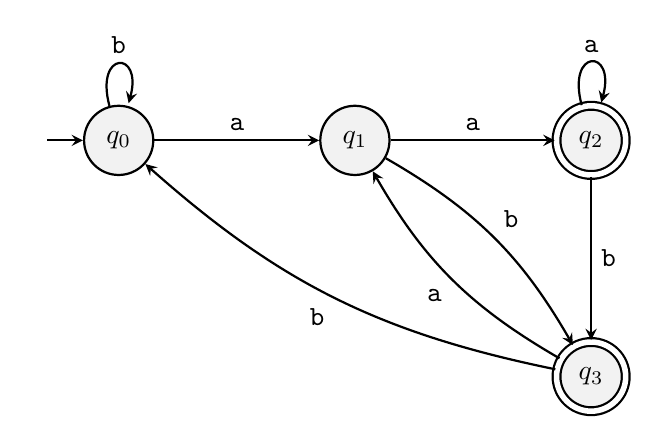
\begin{tikzpicture}
            \node[state, initial] (q0) {$q_0$};
            \node[state, right of=q0] (q1) {$q_1$};
            \node[state, accepting, right of=q1] (q2) {$q_2$};
            \node[state, accepting, below of=q2] (q3) {$q_3$};
            
            \draw (q0) edge[loop above] node {\tt b} (q0);
            \draw (q0) edge node {\tt a} (q1);
            \draw (q1) edge[above] node {\tt a} (q2);
            \draw (q1) edge[bend left] node {\tt b} (q3);
            \draw (q3) edge[bend left] node {\tt a} (q1);
            \draw (q2) edge[loop above] node {\tt a} (q2);
            \draw (q2) edge[right] node {\tt b} (q3);
            \draw (q3) edge[bend left] node {\tt b} (q0);
        \end{tikzpicture}
        \caption{$A_1$: Finite Automaton for $L_1$ }
        \label{fig:state-machine-l1}
    \end{figure}
    
    \begin{figure}[ht] % ’ht’ tells LaTeX to place the figure ’here’ or at the top of the page
        \centering % centers the figure
        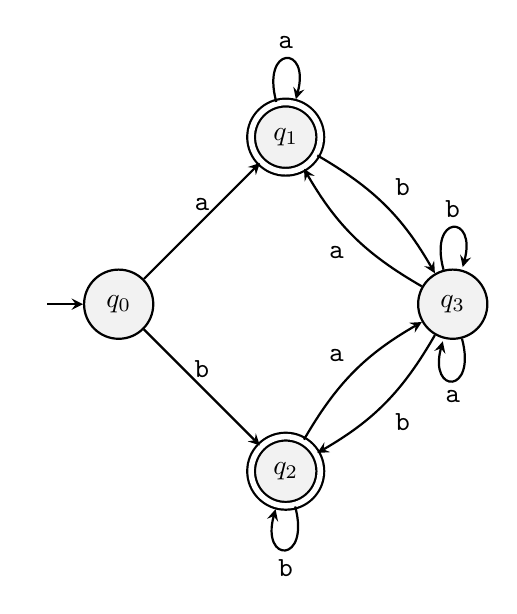
\begin{tikzpicture}
            \node[state, initial] (q0) {$q_0$};
            \node[state, accepting, above right of=q0] (q1) {$q_1$};
            \node[state, accepting, below right of=q0] (q2) {$q_2$};
            \node[state, below right of=q1] (q3) {$q_3$};

            \draw (q0) edge[above] node {\tt a} (q1);
            \draw (q0) edge[above] node {\tt b} (q2);
            
            \draw (q1) edge[loop above] node {\tt a} (q1);
            \draw (q2) edge[loop below] node {\tt b} (q2);
            
            \draw (q1) edge[bend left] node {\tt b} (q3);
            \draw (q3) edge[bend left] node {\tt a} (q1);
            \draw (q2) edge[bend left] node {\tt a} (q3);
            \draw (q3) edge[bend left] node {\tt b} (q2);

            \draw (q3) edge[loop above] node {\tt b} (q3);
            \draw (q3) edge[loop below] node {\tt a} (q3);

            
        \end{tikzpicture}
        \caption{$A_2$: Finite Automaton for $L_2$ }
        \label{fig:state-machine-l2}
    \end{figure}

    \item {Describe the automata from exercise (b) as a five-tuple.}
        \begin{equation*}
            \begin{gathered}
                        \text{\underline{Automata description of $L_1$ as per Figure \ref{fig:state-machine-l1}}}: \\
                        A_1 = (Q_1 , \Sigma , \delta_1 , Q_1^{init} , F_1) \\
                        Q_1 = \{ q_0, q_1, q_2, q_3 \} \\
                        \Sigma = \{ a, b \} \\
                        \delta_1 = \{ (q_0, b, q_0), (q_0, a, q_1), (q_1, a, q_2),  (q_2, a, q_2), (q_2, b, q_3), (q_3, a, q_1), (q_1, b, q_3), (q_3, b, q_0)\} \\
                        Q_1^{init} = \{ q_0 \} \\
                        F_1 = \{ q_2, q_3 \}
            \end{gathered}
        \end{equation*}

        \begin{equation*}
            \begin{gathered}
                \text{\underline{Automata description of $L_2$ as per Figure \ref{fig:state-machine-l2}}}: \\
                A_2 = (Q_2 , \Sigma , \delta_2 , Q_2^{init} , F_2) \\
                Q_2 = \{ q_0, q_1, q_2, q_3 \} \\
                \Sigma = \{ a, b \} \\
                \delta_2 = \{ (q_0, a, q_1),
                            (q_1, a, q_1), (q_0, b, q_2),(q_2, b, q_2),(q_1, b, q_3),(q_3, a, q_1),(q_2, a, q_3),(q_3,a, q_3),(q_3, b, q_3),
                \} \\
                Q_2^{init} = \{ q_0 \} \\
                F_2 = \{ q_1, q_2 \}
            \end{gathered}
        \end{equation*}
\end{enumerate}


\end{document}